\scanpage{77}
connexe, dont le $\pi_1$ est isomorphe en tant que \uline{groupe extérieur}) :
\diagram{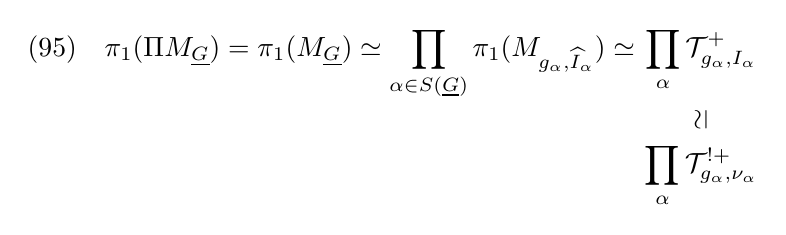
\begin{tikzpicture}[every node/.style={inner sep=0pt}]
\node[anchor=base east] (chain) at (0,0) {$\displaystyle(95)\quad\pi_1(\Pi M_{\underline G})=\pi_1(M_{\underline G})\simeq\prod_{\alpha\in S(\underline G)}\pi_1(M_{g_\alpha,\widehat I_\alpha})\simeq$};
\node[anchor=base west] (upper) at (0.12,0) {$\displaystyle\prod_\alpha\mathcal T^+_{g_\alpha,I_\alpha}$};
\node[rotate=90] at ([yshift=-0.35cm]upper.south) {$\simeq$};
\node[anchor=north] at ([yshift=-0.65cm]upper.south) {$\displaystyle\prod_\alpha\mathcal T^{!+}_{g_\alpha,\nu_\alpha}$};
\end{tikzpicture}}
\margin{où les $\mathcal T^{!+}_{g,\nu}$ sont des groupes de Teichmüller}
Les opérations de $\Gamma^{\unsure{!|\natural|\deleted{!}}}_{\underline G}$ sur $\Pi M_{\underline G}$ définissent un groupoïde mixte $(\Pi M_{\underline G},\Gamma_G)$, dont le groupe fondamental (extérieur) \unsure{s'insère} \deleted{de \unsure{par}} \inserted{dans} une structure d'extension
\[
(96)\quad1\longrightarrow\pi_1(\Pi M_{\underline G},\Gamma_{\underline G})\longrightarrow\pi_1(\Pi M_{\underline G},\Gamma_{\underline G})\relbar\joinrel\relbar\Gamma_G\longrightarrow1
\]
Nous allons définir une \inserted{sorte de} variance des $\Pi M_{\underline G}$ relativement à deux sortes de ``morphismes'' pour les MD-graphes $\underline G$. 

Tout d'abord une \uline{``variance de générisation''}, qui est composée de la \uline{variance pour isomorphismes} de MD-graphes (que j'admets comme ``triviale'', et qu'il est inutile de préciser) et une ``variance de passage au \unsure{quotient} de MD-graphes''.
\margin{76}
